\section{Эксперименты с нейронными сетями}

В данной главе хочется представить исследования о применении машинного обучения
к задаче автоматической тракскрипции музыки. В частности речь пойдет о
нейронных сетях.

В первую очередь стоит определиться с решаемой задачей.
Пусть $x_0^t$ означает последовательность фреймов, каждый из которых
представляет активации(наличие в звуковом спектре)
тех или иных частот в данной время. Это может быть спектрограмма или
постоянное преобразование Q (CQT) от входного аудио потока.
Использую входные данные, необходимо предсказать нотную последовательность
$y_0^t$. Самая распостраненная форма вывода это MIDI тона, то есть
12 значений на октаву или тоже, что одно значение на шаг в клафишах фортепиано.

Допустим имеется система $f: x_0^t \mapsto y_0^t$. И $f$ распознает ноты
в аудио сигналах. Для оценки производительности мы рассмотрим
$X = \{{x_0 ^t}_j\}, Y = \{{y_0^t}_j\}$ - входные данные и желаемый результат
соответственно. $Y_{pred}=f(X)=\{f({x_0^t}_j)\}$ - предсказанные данные
или просто выход системы $f$. Точность работы или производительность
обычно измеряется некоторой метрикой $h$, которая удовлетворяет условиям:
\[
  \forall h: (Y_{pred}, Y) \mapsto \mathbb{R}_{+}
\]
\[
  Y_{pred} = Y \iff h(Y_{pred}, Y) = 0, \text{ иначе } h(Y_{pred}, Y) > 0
\]

Давайте рассмотрим несколько полезных определений из литературы по
машинному обучению.

$TP$ - истинно положительное предсказание события, $FP$ -  ложно положительное
предсказание события, $FN$ - ложно отрицательное предсказание события.

В указанных терминах определяют следующие метрики:
\begin{enumerate}
  \item R (от англ. recall) это мера истинно положительных предсказаний среди всех
    возможных истинно положительных предсказаний.
    \[
      R = \frac{TP}{TP + FN}
    \]
  \item P (от англ. precision) это мера истинно положительных предсказаний
    среди всех истинных предсказаний.
    \[
      P = \frac{TP}{TP + FP}
    \]
  \item F это мера отражающая сбалансированную величину относительно P и R.
    \[
      F = \frac{2 P \cdot R}{P + R}
    \]
\end{enumerate}

P отражает порцию верных предсказаний среди всех произведенных, но не оценивает
покрытие всего множества истинно положительных предсказаний.

R в свою очередь гарантирует покрытие множества истинно положительных
предсказаний, но не оценивает точность самих предсказаний.

Разумно взять меру, которая балансирует эти обе велечины, ведь нам нужна
точная система, которая и распознает хорошо ноты и не оставляет пропущенных.

В машинном обучении существует множество методов для моделирования системы
$f$, которые состоят из выбора архитектуры системы и её оптимизации
для удовлетворения целевой функции точности.

Обычно обучение строиться на обработке данных и подготовке на их основе
тренировочной и тестовой выборок. Тренировочные данные применяются
для решения задач оптимизации моделей, а тестовые данные используются сугубо
для валидации точности и предпочтительно должны минимально пересекаться
с тренировочными, но при этом иметь те жи принципиальные скрытые зависимости.

Для экспериментов в данной статье был использован датасет MAPS \cite{L:MAPS}.
Его подготовка состояла в обработке аудио wav-файлов для получения
CQT матриц. Параметры преобразования совпадают со статьей \cite{SBETENN},
а именно 36 значений на октаву, всего 252 значения начиная от ноты C1,
шаг сдвига 512 единиц. Также исходные аудио дорожки были предварительно
преобразованы в 16KHz из 44.1KHz.

Выбор конкретных параметров обсуждаться не будет, так как целью ставилось
изучение возможностей нейронных сетей. Но стоит упомянуть, что замена
CQT с одним набором параметров, на два с различными, может увеличить точность.
Так например, низкое разрешение даст высокую точность по времени,
а высокое разрешение --- точность по частоте нот соответственно.
Далее рассматривается случай, когда нейронная сеть принимает
только один столбец CQT на фрейм со сбалансированными параметрами
преобразования отностильно приведенных крайних случаев.

Нейронная сеть представляет собой граф вычислений, в котором вершины
отождествляют собой монотонные функции активации, а дуги указывают
направления её передачи. Отдельно выделяют входной слой --- вершины
в которые передются входные данные, обычно одно число на одну вершину
входного слоя. И выходной слой --- это вершины, активации которых используются
для трактования работы системы и обычно обрабатываются для порождения
желаемого распределения значений в соотвествии с целевой задачей.
Все остальные вершины определеют внутренние слои.

Полносвязным слоем называется преобразование следующего вида:
\[
  h_{l + 1} = g(W_l h_l + b_l),
\]
где $h_l$ и $h_{l + 1}$ это значения активации вершин $l$-ого и  $l+1$-ого слоев,
а $g(W_l h_l + b_l)$ задаёт их функциональную связь.
$W_l$ называется матрицей весов дуг
между слоями $h_l$ и $h_{l + 1}$, $b_l$~--- это смещение. Как видим
в аргумент функции $g$ поступает некоторое афинное преобразование
от параметров $h_l$.
Для добавления нелинейности, функцию $g$ обычно выбирают нелинейной.
Классической является сигмоид:
\[
  g(x) = \sigma (x) = \frac{1}{1 + e^{-x}}
\]
Обычно g(x) обладает свойствами:
\[
  0 \leq  g(x) \leq 1,
\]
но необязательно.

Формально для нейронной сети можно задать начальные значения всем параметрам,
а именно весам $W_l$ и $b_l$, также выбрать функции активации $g$.
Затем согласно некоторой функции потерь,
пр. $m(Y_{pred}, Y) = 1.0 - F(Y_{pred}, Y)$
решить задачу минимизации:
\[
  \text{ Найти $\hat f$, что } \forall X=\{{x_0^t}_j\}, Y=\{{y_0^t}_j\}: \quad
  \hat f = \underset{f}{\text{argmin}}(1 - F(f(X), Y))
\]

Для моделирований последовательностей, существует рекуррентный полносвязный
слой:
\[
  h_{l + 1}^t = g(W_l^g h_l^t + W_l^r h_l^{t - 1} + b_l)
\]

В работе для датасета использовались только следующие наборы из MAPS:
\begin{enumerate}
  \item ISOL/NO - изолированные ноты, то есть каждый аудио файл содержит лишь
    одну ноту
  \item ISOL/TR1(2) - изолированные трели, то есть каждый аудио файл содержит
    две чередующиеся ноты с убывающей длительностью.
  \item ISOL/RAND - каждый аудио файл содержит от 2 до 7 случайных пар нот,
    звучащих одновременно на протяжении всего трека.
\end{enumerate}

Ко всем аудио файлам была соотвествующая транскрипции в формате txt,
содержащая имена нот в формате MIDI, и границы их звучания.

Финальные архитектуры сетей:
\begin{enumerate}
  \item Архитектура нейронной сети была простейшая и состояла
    из одного скрытого полносвязного слоя до 2048 вершин,
    и последующего полносвязного слоя на 88 вершин для классификации
    и выдачи активаций соотвествующих MIDI частот.

  \item Для рекуррентной версии был добавлен промежуточный
    полносвязный рекуррентный слой. Но эксперименты с этой частью не были
    закончены, хотя и был подготовлен соотвествующим образом датасет. Проблема
    заключается в некоторой ошибки, из-за которой сеть не обучается даже
    на одном примере. Поэтому требуются дополнительные исследования.
\end{enumerate}

Из результатов хочется отметить, что используя суммарный датасет на 1.6
миллиона фреймов, первая версия сети за 8 часов на машине с процессором
2x1.6GHz обучилась до значения функции потерь на базе F-меры равного 0.28.

Исходный код работы доступен на сайте \cite{L:music-recognizer}.
Далее приводяться
примеры транскрипции для уже использованных аудио записей в предыдущих
экспериметах --- organ.wav (функция потерь по распознаванию системы
сотавляет 0.43, что выше среднего значения тренировки в 0.28)
и композиция исполненная на флейте \cite{L:daj-ci-boza}.

\begin{figure}
  \centering
    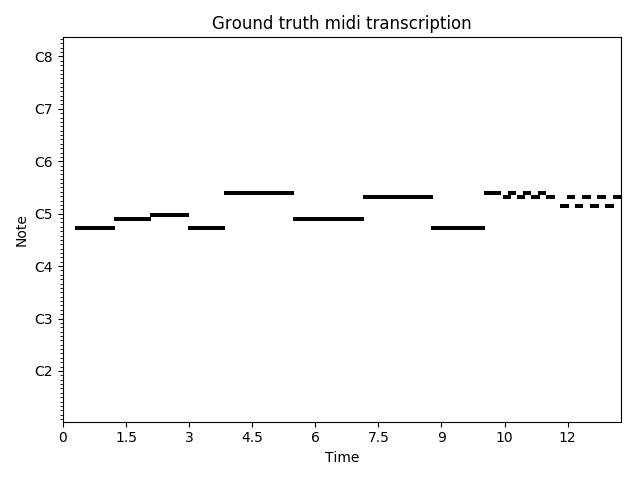
\includegraphics[scale=.8]{res/organ-note-groundtruth.png}
  \centering
  \caption{Исходная транскрипция композиции organ.wav}
    \label{F:organ-notes}
\end{figure}

\begin{figure}
  \centering
    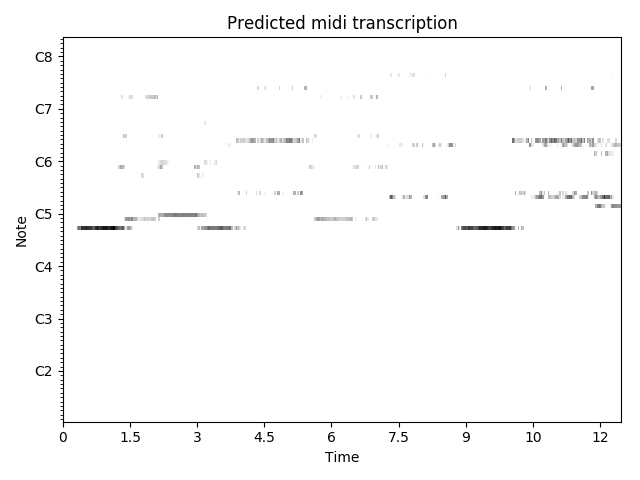
\includegraphics[scale=.8]{res/organ-overfit-028-acoustic.png}
  \centering
  \caption{Результат работы нейронной сети для organ.wav (0.43 значение ошибки)}
    \label{F:organ-pred}
\end{figure}

\begin{figure}
  \centering
    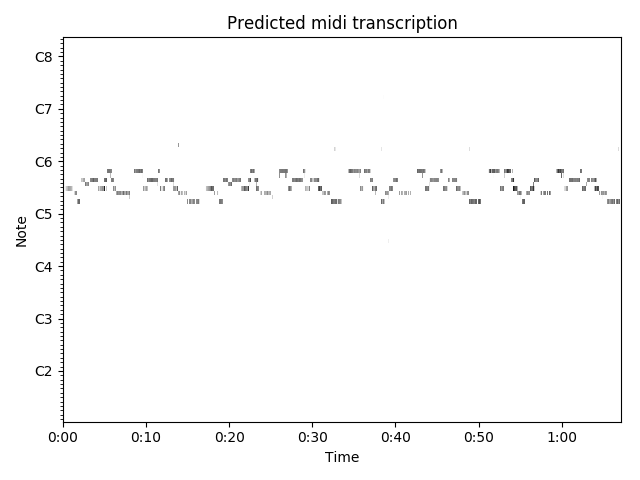
\includegraphics[scale=1]{res/daj-ci-boze-dobranoc-overfit-028-acoustic.png}
  \centering
  \caption{Результат работы нейронной сети для композиции Daj Ce Boze Dobranoc}
    \label{F:daj-pred}
\end{figure}
